\subsubsection{\stid{6.01} LANL ATDM Programming Models and Runtimes}


\paragraph{Overview} 
%\textit{Provide an overview of your project.  You might find that the introductory text from your Fall 2017 Project Summary \url{https://confluence.exascaleproject.org/display/1ST/Fall+2017+ECP+ST+Project+Summaries} useful as a starting draft.}

The LANL ATDM PMR effort is focusing on the development and use of advanced programming models for Advanced Technology Development and Mitigation use-cases. Our current focus is on research and development of new programming model capabilities in the Legion data-centric programming system. Legion provides unique capabilities that align well with our focus on the development of tools and technologies that enables a separation of concerns of computational physicists and computer scientists. Within the ATDM PMR effort we have focused on the development of significant new capabilities within the Legion runtime that are specifically required to support LANL's ATDM applications. Another key component of our work is the co-design and integration of advanced programming model research and development within FleCSI, a Flexible Computational Science Infrastructure.

A major benefit to the broader ECP community is the development of new features in the Legion programming system which are available as free open-source software \url{https://gitlab.com/StanfordLegion/legion}. 


\paragraph{Key  Challenges} \leavevmode \\
%\textit{Describe what is hard to do, why it is challenging.}

\textbf{Legion.}

Applications will face significant challenges in realizing sustained performance on next-generation systems. Increasing system complexity coupled with increasing scale will require significant changes to our current programming model approaches. This is of particular importance for large-scale multi-physics applications where the application itself is often highly dynamic and can exhibit high variability in resource utilization and system bottlenecks depending on what physics are currently in use (or emphasized). Our goal in the LANL ATDM PMR project is to support these highly dynamic applications on Exascale systems, providing improvements in productivity, long-term maintainability, and performance portability of our next-generation applications. 


\textbf{FleCSI Legion integration.}
FleCSI is a Flexible Computational Science Infrastructure whose goal is to provide a common framework for application development for LANL's next-generation codes. FleCSI is required to support a variety of different distributed data structures and computation on these data structures including structured and unstructured mesh as well as mesh-free methods. Our work in the LANL ATDM PMR project is focused on co-designing the FleCSI data and execution model with the Legion programming model to ensure the latest advancements in the programming model and runtimes research community are represented in our computational infrastructure. A significant challenge in our work is the additional constraint that FleCSI must also support other runtime systems such as MPI. Given this constraint, we have chosen an approach that ensures functional correctness across both runtimes but that also leverages and benefits from capabilities in Legion that are not directly supported in MPI (such as task-based parallelism as a first-class construct). 

\paragraph{Solution Strategy} \leavevmode \\
 
%\textit{Describe your basic strategy for addressing the challenges.}

\textbf{Legion.}

In funded collaboration with NVIDIA, LANL and NVIDIA are developing new features in Legion to support our applications. Necessary features are identified through direct engagement with application developers and through rapid development, evaluation, and refactoring within the team. Major features include Dynamic Control Replication for improved scalability and productivity and Dynamic Tracing to reduce runtime overheads for  applications with semi-regular data dependencies such as applications with stencil-based communication patterns. 


\textbf{FleCSI Legion integration.}
LANL staff work on co-design and integration of the Legion programming system into the FleCSI framework. We have regular milestones that align well with application needs and the development of new features within Legion. 


\begin{figure}[htb]
  \centering
  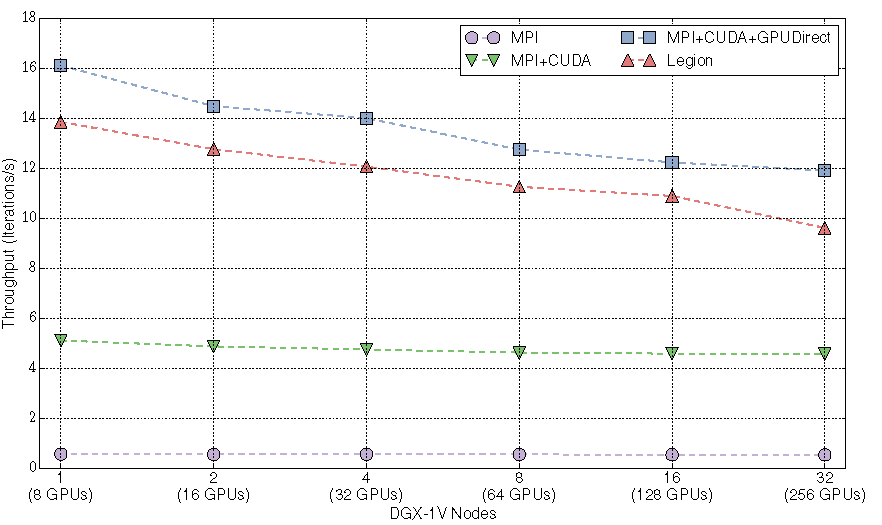
\includegraphics[width=4in]{projects/2.3.6-NNSA/2.3.6.01-LANL-ATDM/control-replication-performance}
        \caption{\label{fig:control-replication-performance}\textbf{Productivity features such as Dynamic Control Replication scales well across multi-GPU systems in unstructured mesh computations.}}
\end{figure}

\begin{figure}[htb]
        \centering
        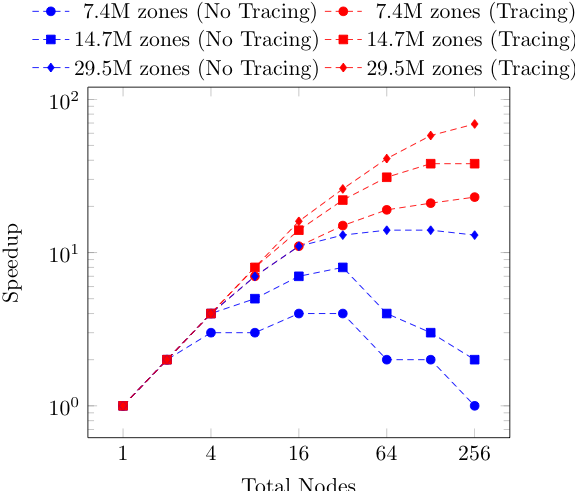
\includegraphics[width=4in]{projects/2.3.6-NNSA/2.3.6.01-LANL-ATDM/tracing-performance}
        \caption{\label{fig:tracing-performance}\textbf{New Legion features such as Tracing will improve strong scaling in unstructured mesh computations.}}
\end{figure}

\paragraph{Recent Progress} \leavevmode \\

%\textit{Describe what you have done recently.  It would be good to have some kind of figure or diagram in this section.}


\textbf{Legion.} 
One of the strengths of Legion is that it executes asynchronous tasks as if they were executed in the sequence they occur in the program. This provides the programmer with a mental model of the computation that is easy to reason about. However, the top-level task in this tree-of-tasks model can often become a sequential bottleneck, as it is responsible for the initial distribution of many subtasks across large machines. In earlier work NVIDIA developed the initial implementation of control replication, which allows the programmer to write tasks with sequential semantics that can be  transparently replicated many times, as directed by the Legion mapper interface, and run in a scalable manner across many nodes.
Dynamic control replication is an important capability for LANL's ATDM effort, allowing our application teams to write applications with apparently sequential semantics while enabling scalability to Exascale architectures. This approach will improve understandability of application code, productivity, and composability of software and ease the burden of optimization and porting to new architectures. 
New dynamic tracing ability has been added to Legion to allow debugging and insight in to peformance optimization activites.

\textbf{FleCSI Legion Integration.} A key component of LANL's Advanced Technology  Development and Mitigation effort is the development of a flexible computational science infrastructure (FleCSI) to support a breadth of application use cases for our Next Generation Code. FleCSI has been co-designed with the Legion programing system in order to enable our Next Generation Code to be performance portable and scalable to future Exascale systems. Legion provides the underlying distributed and node-level runtime environment required for FleCSI to leverage task and data parallelism, data dependent execution, and runtime analysis of task dependencies to expose parallelism. We completed testing of Legion on Sierra with a Visco-Plastic Self-Consistent, VSCP, application to investigate initial performance on GPU systesm.



\paragraph{Next Steps}  \leavevmode \\


\textbf{Legion.} Focus on hardening and scalability of Legion's Dynamic Control Replication and development of Dynamic Tracing for application use-cases. 

\textbf{FleCSI Legion Integration.} Support the Ristra Application milestone to run on Sierra and Trinity.

